\section{Этап Pre-pass} \label{ch3:pre_pass}
	\begin{figure}[ht!] 
		\center
		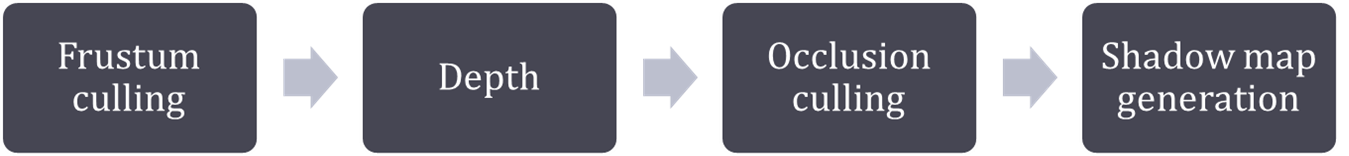
\includegraphics [scale=0.4] {my_folder/images//prepass_schema}	
		\caption{Схема этапа Pre-pass предлагаемого конвеера.} 
		\label{fig:prepass_schema}
	\end{figure}
	
	Во время отрисовки кадра, на разных подэтапах могут требоваться команды, удовлетворяющие разным критериям. Для этого вводится несколько буферов с параметрами команд для ExecuteIndirect, каждый из которых имеет разное имя, работающее как фильтр:
	\begin{enumerate}[1.]
		\item All - буфер, в котором находятся параметры для всех объектов, причутствующих на сцене.
		\item OpaqueAll - буфер, в котором находятся параметры всех непрозрачных объектов.
		\item TransparentAll - буфер, в котором находятся параметры всех прозрачных объектов.
		\item OpaqueFrustum - буфер, в котором находятся параметры всех непрозрачных объектов, пересекающих пирамиду видимости.
		\item OpaqueCulled - буфер, в котором находятся параметры всех непрозрачных объектов, видимых пользователю.
		\item TransparentCulled - буфер, в котором находятся параметры всех прозрачных объектов, видимых пользователю.
	\end{enumerate}
	
	Основной задачей этапа Pre-pass является заполнение всех вышеописанных буферов (кроме All). Разберём подэтапы данного этапа:
	\subsection{Frustum culling} \label{ch3:pre_pass:frustum}
		Данный подэтап отвечает за заполнение буферов OpaqueAll, TransparentAll и OpaqueFrustum при помощи алгоритма под названием Frustum culling\cite{assarsson2000optimized}. Основная идея алгоритма заключается в том, чтобы для каждого объекта преверить, пересекает ли он усеченную пирамиду видимости камеры, или нет (см \firef{fig:frustum_culling}). Если объект и пирамида видимости камеры не пересекаются, то объект можно и не выводить.
		\begin{figure}[ht!] 
			\center
			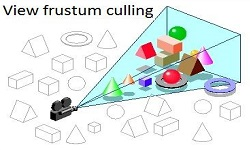
\includegraphics [scale=1] {my_folder/images//frustum_culling}	
			\caption{Схема работы алгоритма Frustum Culling.} 
			\label{fig:frustum_culling}
		\end{figure}
		
		Однако, зачастую, объекты представляют собой сложные невыпуклые геометрические формы, для которых считать пересечения является трудной вычислительной задачей. В связи с этим, в качестве оптимизации, для каждого объекта строится параллельный осям ограничивающий параллелепипед(см. \firef{fig:aabb}), и проверяется пересечение не объектов с усечённой пирамидой видимости, а пересечение параллелепипедов и усечённой пирамиды. 
		
		\begin{figure}[ht!] 
			\center
			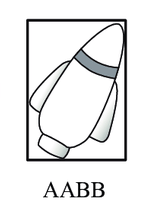
\includegraphics [scale=0.8] {my_folder/images//aabb}	
			\caption{Пример построения параллельного осям ограничивающего параллелепипеда в двухмерном случае.} 
			\label{fig:aabb}
		\end{figure}
		
		Для того чтобы проверить, пересекаются ли параллелипипед и усеченная пирамида, достаточно задать уравнения плоскостей, содержащих грани усеченной пирамиды, и имеющие нормали, направленные \say{внутрь} пирамиды. Предположим, что плоскости задаются уравнениями \ref{eq:frustum_plane}, а вершины параллельного осям ограничивающего параллелепипеда задаются как \ref{eq:aabb_points}.
		
		\begin{equation} % \tag{S} % tag - вписывает свой текст 
			\label{eq:frustum_plane}
			\begin{multlined}
				A_i * x + B_i * y + C_i * z + D = 0, \forallAlt 1 \le i \le 6 
			\end{multlined}
		\end{equation}
		
		\begin{equation} % \tag{S} % tag - вписывает свой текст 
			\label{eq:aabb_points}
			\begin{multlined}
				{x_j, y_j, z_j} \forallAlt 1 \le j \le 8 
			\end{multlined}
		\end{equation}
		
		Тогда выполнение условия \ref{eq:frustum_check} гарантирует то, что объект не попадёт в область видимости.
		
		\begin{equation} % \tag{S} % tag - вписывает свой текст 
			\label{eq:frustum_check}
			\begin{multlined}
				\existsAlt i  \forallAlt j A_i * x_j + B_i * y_j + C_i * z_j + D < 0
			\end{multlined}
		\end{equation}
				
	\subsection{Depth pre-pass} \label{ch3:pre_pass:depth}
		Данный подэтап выполняет задачу построения иерархической карты глубины, используя объекты из буфера OpaqueFrustum.
		
		Для начала, определим что такое карта глубины и что такое иерархическая карта глубины. \textit{Картой глубины} называется монохромное изображение, где для каждого пикселя, вместо интенсивности цвета, хранится его расстояние до камеры.  \textit{Иерархической картой глубины} называется набор монохромных изображений, удовлетворяющих следующим условиям:
		\begin{enumerate}[1.]
			\item Первое изображение совпадает по размеру и содержимому с картой глубины
			\item Ширина и высота каждого следующего изображения меньше ширины и высоты предыдущего в 2 раза
			\item Для каждого следующего изображения, интенсивнось пикселя считается как максимум из четырёх соотвествующих пикселей предыдущего
		\end{enumerate}
	
		\begin{figure}[ht!] 
			\center
			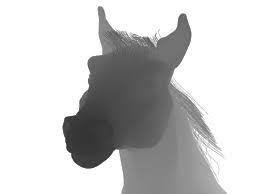
\includegraphics [scale=1] {my_folder/images//depth_map}	
			\caption{Пример карты глубины.} 
			\label{fig:depth_map}
		\end{figure}
		
		\begin{figure}[ht!] 
			\center
			
\includegraphics [scale=1] {my_folder/images//hier_depth_map}	
			\caption{Пример иерархической карты глубины.} 
			\label{fig:hier_depth_map}
		\end{figure}
		\FloatBarrier
		Построение такой карты предоставляет следующие преимущества:
		\begin{enumerate}[1.]
			\item Предварительный подсчёт карты глубины позволяет позднее высчитывать цвет пикселей только тех объектов, для которых рассотояние до камеры совпадает со значением в карте глубины
			\item Построенная иерархическая карты глубины позволяет применить алгоритм Occlusion culling, о котором будет сказано далее
		\end{enumerate}
	\subsection{Occlusion culling} \label{ch3:pre_pass:occlusion}
		Данный подэтап отвечает за заполнение буферов OpaqueCulled и  TransparentCulled при помощи алгоритма Occlusion culling\cite{greene1993hierarchical}. Основная цель данного алгоритма заключается в отбрасывании тех объектов, которые оказываются перекрыты близлежащими объектами (см \firef{fig:occlusion_culling}). 
		
		\begin{figure}[ht!] 
			\center
			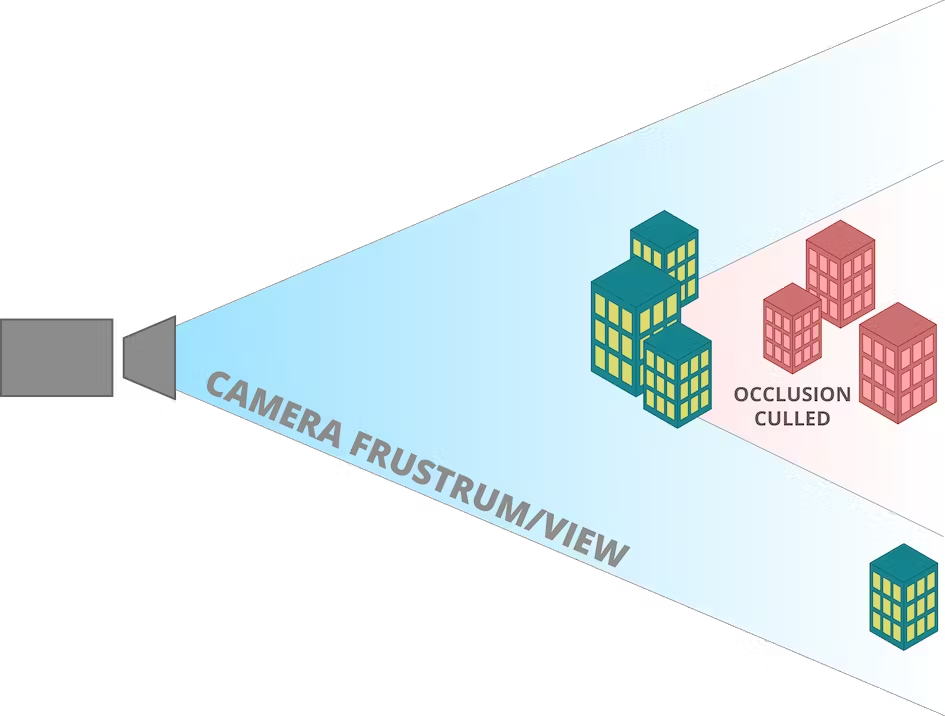
\includegraphics [scale=0.27] {my_folder/images//occlusion_culling}	
			\caption{Схема работы алгорима Occlusion culling.} 
			\label{fig:occlusion_culling}
		\end{figure}
		
		Для этого:
		\begin{enumerate}[1.]
			\item Каждый объект представляется в виде параллельного осям ограничивающего параллелепипеда (см. главу \ref{ch3:pre_pass:frustum})
		 	\item Среди вершин параллелепипеда находится ближайшая, и её расстояние до камеры сохраняется.
		 	\item Каждая вершина параллелепипеда проецируется на экран, тем самым получаются координаты пикселей, соответствующих данной вершине.
		 	\item Вокруг спроецированных вершин строится параллельный осям ограничивающий прямоугольник.
		 	\item По размеру прямоугольника выбирается изображение из иерархической карты глубины (см. главу \ref{ch3:pre_pass:depth}) таким образом, чтобы весь прямоугольник соответствовал одному пикселю изображения.
		 	\item Если интенсивность в соответствующем пикселе изображения из иерархической карты глубины меньше, чем сохранённая глубина - то объект перекрывается другими объектами, и его копировать не надо. 
		 	\item Иначе, объект может быть виден, и тогда его необходимо скопировать в соответсвующий буфер. 
		\end{enumerate}
		
	\subsection{Построение карт теней} \label{ch3:pre_pass:shadow_maps}
		Данный подэтап отвечает за построение карт теней, для реализации алгоритмов затенения\cite{williams1978casting}. Сами по себе карты теней очень похожи на \say{карту глубины} (см главу \ref{ch3:pre_pass:depth}). Основное отличие заключается лишь в том, что в интенсивность записывается расстояние не от камеры до объекта, а от источника света до объекта.
		
		При наличии карты теней, проверить находится ли точка в тени достаточно просто: необходимо лишь посчитать расстояние от точки до источника света, и если оно больше записанного в карте теней, то в данной точке присутствует тень.
		
		Однако, в силу того, что изображение имеет конечное разрешение, при некотором приближении тени могут оказазаться \say{блочными}, как показано на \firef{fig:blocky_shadows}.
		 
		 \begin{figure}[ht!] 
		 	\center
		 	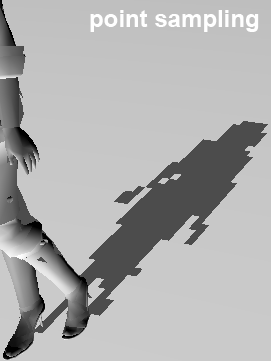
\includegraphics [scale=1] {my_folder/images//blocky_shadows}	
		 	\caption{Пример "блочных" теней.} 
		 	\label{fig:blocky_shadows}
		 \end{figure}
		 
		 Чтобы избежать этого эффекта и необходимости затрачивать большое количество памяти на тени, используется алгоритм Persentage Closure Filtering\cite{fernando2005percentage}. Суть этого алгоритма заключается в том, чтобы сравнивать расстояние от точки до источника света не с одиним пикселем, а с несколькими, рядом-лежащими пикселями. При применении такого подхода, тени становятся \say{мягкими}, как показано на \firef{fig:pcf_shadows}.
		 
		 \begin{figure}[ht!] 
		 	\center
		 	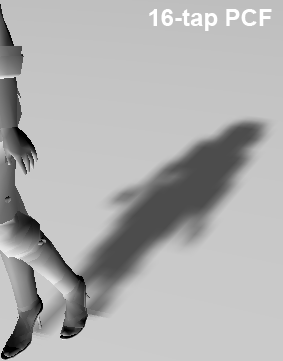
\includegraphics [scale=1] {my_folder/images//pcf_shadows}	
		 	\caption{Пример мягких теней.} 
		 	\label{fig:pcf_shadows}
		 \end{figure}
		 
		 В связи с тем, что невозможно одновременно заполнить карты теней для всех источников света на сцене, этот подэтап требует отрисовки для каждого источника света, генерирующего тень.